\section{Algebra}
\label{sec:algebra}

Calculus will give us new things to do with functions, but we'll still
need our algebra. This chapter collects a few tools we'll use along
the way.

\subsection{Properties of Exponents}
\label{sec:exponent-properties}

Exponents let us write repeated multiplication without writing every
factor. When we multiply powers with the same base, we add their
exponents. When we raise a power to another power, we multiply the
exponents. For positive bases $a$ and $b$ and real numbers $r$ and $s$,
\begin{align*}
a^ra^s&=a^{r+s},
&\frac{a^r}{a^s}&=a^{r-s},\\
(a^r)^s&=a^{rs},
&(ab)^r&=a^rb^r,\\
\left(\frac ab\right)^r&=\frac{a^r}{b^r},
&a^{-r}&=\frac1{a^r}.
\end{align*}
Also, $a^0=1$. A negative exponent tells us to take a reciprocal;
it doesn't make the answer negative.

Fractional exponents tell us to take roots. For an integer $m$ and
a positive integer $n$,
$$a^{m/n}=\left(\sqrt[n]{a}\right)^m=\sqrt[n]{a^m}.$$
We used positive bases so all of these expressions make sense for
real exponents. Negative bases need more care, since some roots
aren't real.

\begin{exampleblock}
For $x,y>0$, let's simplify an expression with several powers:
\begin{align*}
\frac{(x^2y^{-1})^3}{x^{-1}y^2}
&=\frac{x^6y^{-3}}{x^{-1}y^2}
&&\text{(multiply the exponents)},\\
&=x^{6-(-1)}y^{-3-2}
&&\text{(subtract the exponents)},\\
&=\frac{x^7}{y^5}
&&\text{(use positive exponents)}.
\end{align*}
\end{exampleblock}

\begin{exampleblock}
We can evaluate $16^{-3/4}$ without a calculator:
$$16^{-3/4}=\frac1{(\sqrt[4]{16})^3}=\frac1{2^3}=\frac18.$$
\end{exampleblock}

\subsection{Properties of Logarithms}

Remember that a logarithm tells us an exponent. For $b>0$, $b\ne1$,
and $u>0$,
$$\log_b(u)=s\quad\Longleftrightarrow\quad b^s=u.$$
In other words, logarithms and exponentials undo each other:
$$b^{\log_b(u)}=u,\qquad \log_b(b^s)=s.$$
In particular, $\log_b(1)=0$ and $\log_b(b)=1$.

The properties of logarithms come from the
\hyperref[sec:exponent-properties]{properties of exponents}.
Multiplying powers adds their exponents, so taking the logarithm of
a product should give us a sum.

\begin{thm}[Properties of Logarithms]
\proofref{proof:logarithm-rules}
For $b>0$, $b\ne1$, $u,v>0$, and any real number $r$,
\begin{align*}
\log_b(uv)&=\log_b(u)+\log_b(v)
&&\text{(product property)},\\
\log_b(u/v)&=\log_b(u)-\log_b(v)
&&\text{(quotient property)},\\
\log_b(u^r)&=r\log_b(u)
&&\text{(power property)}.
\end{align*}
For another base $c>0$, $c\ne1$, the \textbf{change-of-base formula} is
$$\log_b(u)=\frac{\log_c(u)}{\log_c(b)}.$$
\end{thm}

These properties work for $\ln$, since $\ln=\log_e$. They let us split
up logarithms of products, quotients, and powers, but not sums:
$\log_b(u+v)$ does not generally equal $\log_b(u)+\log_b(v)$.
\mar{Use the change-of-base formula to write $\log_2(7)$ using $\ln$.}

\begin{exampleblock}
For $x>1$, we can expand
\begin{align*}
\ln\left(\frac{x^2\sqrt{x+1}}{(x-1)^3}\right)
&=\ln(x^2)+\ln\bigl((x+1)^{1/2}\bigr)-\ln\bigl((x-1)^3\bigr)\\
&=2\ln(x)+\frac12\ln(x+1)-3\ln(x-1).
\end{align*}
The condition $x>1$ makes every logarithm here defined.
\end{exampleblock}

Be careful with signs when using the power property. Although $\ln(x^2)$
is defined for every $x\ne0$, $2\ln(x)$ is only defined for $x>0$.
Since $x^2=|x|^2$, the version that works for every $x\ne0$ is
$$\ln(x^2)=2\ln|x|.$$

\begin{exampleblock}
Let's solve $\log_2(x-1)+\log_2(x+1)=3$. First, both logarithms
must be defined, so $x>1$. Then
\begin{align*}
\log_2\bigl((x-1)(x+1)\bigr)&=3
&&\text{(combine the logarithms)},\\
x^2-1&=2^3
&&\text{(rewrite as an exponential)},\\
x^2&=9.
\end{align*}
The algebra gives $x=\pm3$, but only $x=3$ satisfies $x>1$.
\end{exampleblock}

\subsection{The Binomial Theorem}

A \textbf{binomial} is a sum of two terms. We already know how to
square one: $(a+b)^2=a^2+2ab+b^2$. The Binomial Theorem tells us
how to expand any nonnegative integer power without multiplying
everything out by hand.

First, we need some notation. For a positive integer $n$, its
\textbf{factorial} is $n!=1\cdot2\cdots n$. We also define $0!=1$.
The \textbf{binomial coefficient}
$$\binom nk=\frac{n!}{k!(n-k)!},\qquad k=0,1,\ldots,n,$$
is read ``$n$ choose $k$.'' It counts the ways to choose $k$ objects
from $n$ objects, when the order doesn't matter.

\begin{thm}[Binomial Theorem]
\proofref{proof:binomial-theorem}
For a nonnegative integer $n$ and real numbers $a$ and $b$,
$$(a+b)^n=\sum_{k=0}^n\binom nk a^{n-k}b^k.$$
\end{thm}

As $k$ goes from 0 to $n$, the power of $a$ goes down and the power
of $b$ goes up. The sum of their exponents is always $n$.

A quick way to get the coefficients is \textbf{Pascal's triangle}.
Start with a 1 at the top. Each new row begins and ends with 1;
every number in between is the sum of the two numbers just above it.
Count the top row as $n=0$. Row $n$ gives the coefficients of
$(a+b)^n$, in order.

\begin{figure}[H]
\centering
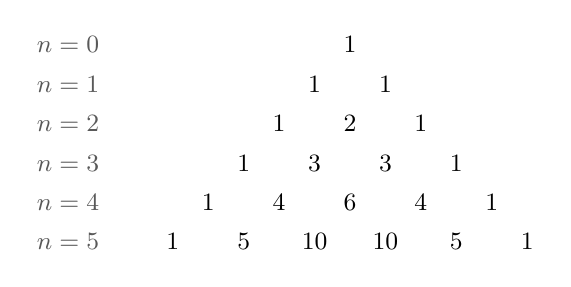
\begin{tikzpicture}[x=9mm,y=5mm,every node/.style={font=\small}]
\foreach \n/\entries in {0/{1},1/{1,1},2/{1,2,1},3/{1,3,3,1},
                         4/{1,4,6,4,1},5/{1,5,10,10,5,1}} {
  \node[anchor=east,text=black!65] at (-3.4,-\n) {$n=\n$};
  \foreach \entry [count=\k from 0] in \entries
    \node at ({\k-\n/2},-\n) {$\entry$};
}
\end{tikzpicture}

\caption{Pascal's Triangle}
\label{fig:pascal-triangle}
\end{figure} \mar{Make sure you understand where the 6 comes from. Then add the $n=6$ row.}

\begin{exampleblock}
To expand $(1+x)^4$, use $a=1$, $b=x$, and $n=4$:
\begin{align*}
(1+x)^4
&=\binom40+\binom41x+\binom42x^2+\binom43x^3+\binom44x^4\\
&=1+4x+6x^2+4x^3+x^4.
\end{align*}
For instance, the coefficient of $x^2$ is
$\binom42=4!/(2!2!)=6$.
We can also read all five coefficients, $1,4,6,4,1$, directly from
row $n=4$ of Pascal's triangle in Figure~\ref{fig:pascal-triangle}.
\end{exampleblock}

\subsection{Completing the Square}

\textbf{Completing the square} rewrites a quadratic using a squared
binomial. The idea comes from expanding
$$(x+h)^2=x^2+2hx+h^2.$$
To match the linear term in $x^2+bx$, choose $h=b/2$. Then add and
subtract $(b/2)^2$ so we haven't changed the expression:
\begin{align*}
x^2+bx+c
&=x^2+bx+\left(\frac b2\right)^2
  -\left(\frac b2\right)^2+c\\
&=\left(x+\frac b2\right)^2+c-\frac{b^2}{4}.
\end{align*}
If the coefficient of $x^2$ isn't 1, factor it out of the quadratic
and linear terms first. For $a\ne0$, this gives
$$ax^2+bx+c
=a\left(x+\frac{b}{2a}\right)^2+c-\frac{b^2}{4a}.$$

\begin{exampleblock}
Let's complete the square in $2x^2-12x+5$:
\begin{align*}
2x^2-12x+5
&=2(x^2-6x)+5 &&\text{(factor out 2)},\\
&=2(x^2-6x+9-9)+5 &&\text{(half of $-6$ is $-3$)},\\
&=2\bigl((x-3)^2-9\bigr)+5 &&\text{(make the square)},\\
&=2(x-3)^2-13.
\end{align*}
This form tells us that the smallest value is $-13$, which occurs
when $x=3$.
\end{exampleblock}

\begin{exampleblock}
We can also use this to solve $x^2+6x+2=0$:
\begin{align*}
x^2+6x&=-2,\\
x^2+6x+9&=7 &&\text{(add $(6/2)^2$ to both sides)},\\
(x+3)^2&=7,\\
x&=-3\pm\sqrt7.
\end{align*}
Remember to include both signs when taking the square root.
\end{exampleblock}
